% Options for packages loaded elsewhere
\PassOptionsToPackage{unicode}{hyperref}
\PassOptionsToPackage{hyphens}{url}
%
\documentclass[
]{book}
\title{A Minimal Book Example}
\author{John Doe}
\date{2021-12-01}

\usepackage{amsmath,amssymb}
\usepackage{lmodern}
\usepackage{iftex}
\ifPDFTeX
  \usepackage[T1]{fontenc}
  \usepackage[utf8]{inputenc}
  \usepackage{textcomp} % provide euro and other symbols
\else % if luatex or xetex
  \usepackage{unicode-math}
  \defaultfontfeatures{Scale=MatchLowercase}
  \defaultfontfeatures[\rmfamily]{Ligatures=TeX,Scale=1}
\fi
% Use upquote if available, for straight quotes in verbatim environments
\IfFileExists{upquote.sty}{\usepackage{upquote}}{}
\IfFileExists{microtype.sty}{% use microtype if available
  \usepackage[]{microtype}
  \UseMicrotypeSet[protrusion]{basicmath} % disable protrusion for tt fonts
}{}
\makeatletter
\@ifundefined{KOMAClassName}{% if non-KOMA class
  \IfFileExists{parskip.sty}{%
    \usepackage{parskip}
  }{% else
    \setlength{\parindent}{0pt}
    \setlength{\parskip}{6pt plus 2pt minus 1pt}}
}{% if KOMA class
  \KOMAoptions{parskip=half}}
\makeatother
\usepackage{xcolor}
\IfFileExists{xurl.sty}{\usepackage{xurl}}{} % add URL line breaks if available
\IfFileExists{bookmark.sty}{\usepackage{bookmark}}{\usepackage{hyperref}}
\hypersetup{
  pdftitle={A Minimal Book Example},
  pdfauthor={John Doe},
  hidelinks,
  pdfcreator={LaTeX via pandoc}}
\urlstyle{same} % disable monospaced font for URLs
\usepackage{longtable,booktabs,array}
\usepackage{calc} % for calculating minipage widths
% Correct order of tables after \paragraph or \subparagraph
\usepackage{etoolbox}
\makeatletter
\patchcmd\longtable{\par}{\if@noskipsec\mbox{}\fi\par}{}{}
\makeatother
% Allow footnotes in longtable head/foot
\IfFileExists{footnotehyper.sty}{\usepackage{footnotehyper}}{\usepackage{footnote}}
\makesavenoteenv{longtable}
\usepackage{graphicx}
\makeatletter
\def\maxwidth{\ifdim\Gin@nat@width>\linewidth\linewidth\else\Gin@nat@width\fi}
\def\maxheight{\ifdim\Gin@nat@height>\textheight\textheight\else\Gin@nat@height\fi}
\makeatother
% Scale images if necessary, so that they will not overflow the page
% margins by default, and it is still possible to overwrite the defaults
% using explicit options in \includegraphics[width, height, ...]{}
\setkeys{Gin}{width=\maxwidth,height=\maxheight,keepaspectratio}
% Set default figure placement to htbp
\makeatletter
\def\fps@figure{htbp}
\makeatother
\setlength{\emergencystretch}{3em} % prevent overfull lines
\providecommand{\tightlist}{%
  \setlength{\itemsep}{0pt}\setlength{\parskip}{0pt}}
\setcounter{secnumdepth}{5}
\usepackage{booktabs}
\ifLuaTeX
  \usepackage{selnolig}  % disable illegal ligatures
\fi
\usepackage[]{natbib}
\bibliographystyle{plainnat}

\begin{document}
\maketitle

{
\setcounter{tocdepth}{1}
\tableofcontents
}
\hypertarget{arbeidskrav1}{%
\chapter{Arbeidskrav1}\label{arbeidskrav1}}

\hypertarget{introduksjon}{%
\section{Introduksjon}\label{introduksjon}}

En av de mest sentrale faktorene for utholdenhets prestasjonen er det maksimale oksygenopptaket (VO2maks) \citet{bassett2000}. VO2maks er bestemt av flere sentrale faktorer: lungenes kapasitet til å føre oksygen fra blodet, hjertets pumpekapasitet, volum, og sammensetning av blodet, og musklenes evne til å bruke oksygenet \citet{bassett2000}.

Reliabilitet kan bli definert som reproduserbarheten til testverdier, analyser eller andre målinger på gjentatte forsøk på de samme individene. Det finnes tre hoved variasjoner man må ta hensyn til når man snakker om reliabilitet, det er: deltakernes variasjon, endring i gjennomsnittet og rettest korrelasjon \citet{hopkins2000}. Deltakernes variasjon regnes ut gjennom standardavvik og standardfeil. Det kan komme fra biologiske forhold som kan variere mellom to tester. Utstyr kan og spille inn på dette, hvor det er støy ved målingene. Endring i gjennomsnitt kan man dele i to deler, det er tilfeldig endring og systematisk endring. Tilfeldig endring er støy i målinger og data innsamlingsfeil. Dette kan minimeres gjennom å ha mange tester, hvor da tilfeldige feilene vil spille mindre inn på resultatet. Systematisk endring er treningseffekten og læringseffekten man kan forvente mellom to tester, det handler om faktorene som spiller inn og kan gjøre test2, bedre enn test1. Korrelasjon i test2 handler om hvor godt test1 og test2 korrelerer, hvis man har bedre korrelasjon, har man og høyere reliabilitet mellom testene.

\hypertarget{metode}{%
\section{Metode}\label{metode}}

I denne rapporten skal reliabiliteten estimeres mellom to VO2maks tester. Hvor test1 og test2 er gjennomført med en ukes mellomrom.

VO2maks testen ble gjennomført med en standard VO2maks protokoll. Hvor stigningen var konstant, 10,5\% for guttene og 5,5\% for jentene. Startfart var gitt på forhånd hvor alle startet på 8 km/t. For hvert minutt som gikk, økte farten med 1 km/t, og slik fortsatte det til utmattelse. Underveis i testen ble det gitt verbal oppmuntring fra testleder, det var og testleder som justerte farten underveis. Testen ble gjennomført på en woodway løpemølle (4FRONT, wisconsin). Hele testen ble gjennomført med kontinuerlig oksygenmåling hvert 30. sekund. Oksygenmålingene ble gjennomført med en Vyntus CPX, mixing chamber (Vyntus CPX, Jaeger-CareFusion, UK). Ved målinger på Vyntus CPX ble det automatisk kalibrert for gass, volum og luftfuktighet før hver test. Oppvarmingen før testen var valgfri, og varte i 15 min. Underveis i oppvarmingen ble testprotokollen forklart for utøver, og eventuelle spørsmål om testen ble avklart. Under testen ble det registrert ml/min VO2. Umiddelbart etter testen ble det spurt om Borg skala 6-20 (RPE: \citet{borg1970} ), det ble og notert ned hva siste belastning var og hvor lenge utøver løp på denne belastningen. Et minutt etter testen ble det målt laktat (La) gjennom et fingerstikk og analysert gjennom Biosen blodlaktatmåler (Biosen C-line, EKF Diagnostics, Barleben, Germany), HF ble og notert ned.

Test2 ble gjennomført på samme måte som test1, hvor samme protokoll ble gjennomført på nytt.

\hypertarget{statistikk}{%
\section{Statistikk}\label{statistikk}}

Alle statistiske beregninger ble gjort i RStudio (versjon RStudio 1.4.1717; R Foundation for Statistics Computing, Vienna, AT). Det ble regnet ut gjennomsnitt og standardavvik mellom test1 og test2. Det ble også regnet ut standardfeil for testen som et mål på reliabilitet.

\hypertarget{resultat-og-diskusjon}{%
\section{Resultat og diskusjon}\label{resultat-og-diskusjon}}

Resultatene for studien er vist i figur 1.

Standardfeilen i studien var 4.04 \%.

Standardaviket i studien var 229.82

\begin{figure}
\centering
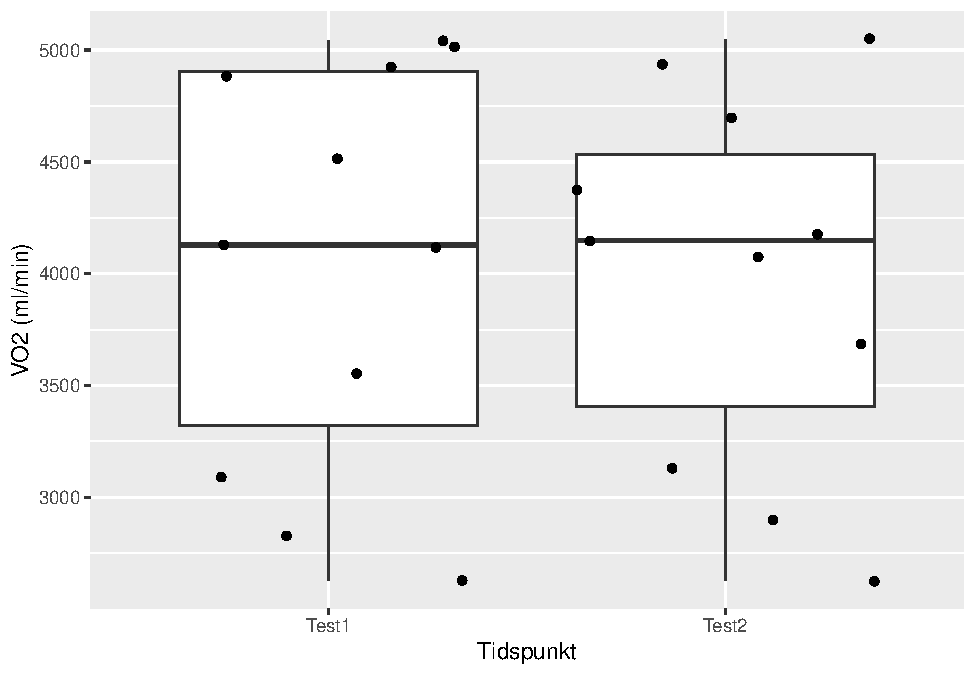
\includegraphics{_main_files/figure-latex/unnamed-chunk-2-1.pdf}
\caption{\label{fig:unnamed-chunk-2}Figur 1 viser resultater fra test 1 og 2}
\end{figure}

\hypertarget{vitenskapsfilosofi}{%
\chapter{Vitenskapsfilosofi}\label{vitenskapsfilosofi}}

Placeholder

\hypertarget{falsifikasjonisme}{%
\section{Falsifikasjonisme}\label{falsifikasjonisme}}

\hypertarget{hd-metoden-og-abduksjonbayesisme}{%
\section{HD-metoden og abduksjon/Bayesisme}\label{hd-metoden-og-abduksjonbayesisme}}

\hypertarget{replikasjonskrisen}{%
\section{Replikasjonskrisen}\label{replikasjonskrisen}}

\hypertarget{study-design}{%
\chapter{Study-Design}\label{study-design}}

Placeholder

\hypertarget{inntroduksjon}{%
\section{Inntroduksjon}\label{inntroduksjon}}

\hypertarget{metode-1}{%
\section{Metode}\label{metode-1}}

\hypertarget{analyzing-repeated-measures-experiments}{%
\chapter{Analyzing repeated measures experiments}\label{analyzing-repeated-measures-experiments}}

Placeholder

\hypertarget{inntroduksjon-1}{%
\section{Inntroduksjon}\label{inntroduksjon-1}}

\hypertarget{metode-2}{%
\section{Metode}\label{metode-2}}

\hypertarget{forsuxf8kspersoner}{%
\subsection{Forsøkspersoner}\label{forsuxf8kspersoner}}

\hypertarget{treningsprotokol}{%
\subsection{Treningsprotokol}\label{treningsprotokol}}

\hypertarget{statestikk}{%
\subsection{Statestikk}\label{statestikk}}

\hypertarget{resultater}{%
\section{Resultater}\label{resultater}}

\hypertarget{diskusjon}{%
\section{Diskusjon}\label{diskusjon}}

\hypertarget{konklusjon}{%
\subsection{Konklusjon}\label{konklusjon}}

\hypertarget{footnotes-and-citations}{%
\chapter{Footnotes and citations}\label{footnotes-and-citations}}

\hypertarget{footnotes}{%
\section{Footnotes}\label{footnotes}}

Footnotes are put inside the square brackets after a caret \texttt{\^{}{[}{]}}. Like this one \footnote{This is a footnote.}.

\hypertarget{citations}{%
\section{Citations}\label{citations}}

Reference items in your bibliography file(s) using \texttt{@key}.

For example, we are using the \textbf{bookdown} package \citep{R-bookdown} (check out the last code chunk in index.Rmd to see how this citation key was added) in this sample book, which was built on top of R Markdown and \textbf{knitr} \citep{xie2015} (this citation was added manually in an external file book.bib).
Note that the \texttt{.bib} files need to be listed in the index.Rmd with the YAML \texttt{bibliography} key.

The RStudio Visual Markdown Editor can also make it easier to insert citations: \url{https://rstudio.github.io/visual-markdown-editing/\#/citations}

\hypertarget{blocks}{%
\chapter{Blocks}\label{blocks}}

Placeholder

\hypertarget{equations}{%
\section{Equations}\label{equations}}

\hypertarget{theorems-and-proofs}{%
\section{Theorems and proofs}\label{theorems-and-proofs}}

\hypertarget{callout-blocks}{%
\section{Callout blocks}\label{callout-blocks}}

\hypertarget{sharing-your-book}{%
\chapter{Sharing your book}\label{sharing-your-book}}

Placeholder

\hypertarget{publishing}{%
\section{Publishing}\label{publishing}}

\hypertarget{pages}{%
\section{404 pages}\label{pages}}

\hypertarget{metadata-for-sharing}{%
\section{Metadata for sharing}\label{metadata-for-sharing}}

  \bibliography{book.bib,packages.bib}

\end{document}
